\newif\ifglobal

%%%%%%%%%%%%%%%%%%%%%%%
%%% Compile to view %%%
%%%%%%%%%%%%%%%%%%%%%%%

%%%%%%%%%%%%%%%%%%%%%%%%%%%%%%%%%%%%%%%%%%%%%%%%%%%
%%% Readme:                                     %%%
%%% https://www.overleaf.com/read/bwdjvfjksvjy/ %%%
%%%%%%%%%%%%%%%%%%%%%%%%%%%%%%%%%%%%%%%%%%%%%%%%%%%

% >>> M?: marks a module setting number or important notice

% >>> M4: Set {./relative-path} to external files for this module <<<
\def \modulefiles {./25-SENSOR}
% To add an external file, use:
% (Replace '---' with actual filename)
% '\input{\modulefiles/tables/---.tex}' for tables
% '\includegraphics{\modulefiles/figures/---}' for figures
% '\subfile{\modulefiles/---}' for register files

% >>> M1: This module is in global project? <<<
% 'YES' - uncomment; 'NO' - comment out
\globaltrue

\ifglobal
    \documentclass[main\_\_EN.tex]{subfiles}

\else
    \documentclass[openany, 10pt]{book}

    % >>> M2: In ./00-shared/preamble-trm-module, also find
    %         settings for visibility of todo notes, watermark <<<
    \usepackage{preamble-trm-module}

    % >>> M3: Temporary labels in English,
    %         you can add your own labels there <<<
    \myexternaldocument{./00-shared/temp-labels-en}

\fi %\ifglobal


\setcounter{secnumdepth}{4}

% >>> M5: If this module needs any updates in
% './00-shared/preamble-trm-module.sty'
% (include additional package, etc.), contact your module PM
% or create the file './00-shared/changelog.tex' make the
% necessary updates yourself and document them in this file <<<


\begin{document}


% Sets language into which pre-defined bits of text are translated
\selectlanguage{english}

% Do not delete this block
\ifglobal
% Add the following front matter if
% this module is outside of global project
\else
    \InputIfFileExists{readme}{}{}
    {\let\clearpage\relax \listoftodos}
    \tableofcontents
    %\listoftables
    %\listoffigures
\fi


%%%%%%%%%%%%%%%%%%%%%%%%%
%%% TRM Module Begins %%%
%%%%%%%%%%%%%%%%%%%%%%%%%

\hypertarget{sensor}{}
\chapter{On-Chip Sensors and Analog Signal Processing}
\label{mod:sensor}

\section{Overview} \label{subsection:on-chip-sensor-overview}

\chipname{} provides the following on-chip sensors and signal processing peripherals:

\begin{itemize}
\item Fourteen \hyperref[ssec:touch sensor]{capacitive touch sensors} that can be used to detect finger touches from 14 channels. The touch sensors can also be configured to be moisture tolerant, and support Water Rejection capabilities. A proximity sensing mode is also supported.

\item One temperature sensor for measuring the internal temperature of the \chipname{} chip.
\item Two 12-bit Successive Approximation ADCs (SAR ADCs) controlled by five dedicated controllers that can input analog signals from total of 20 channels. The SAR ADCs can operate in a high-performance mode or a low-power mode.
\end{itemize}

\section{Capacitive Touch Sensors}\label{ssec:touch sensor}

\subsection{Terminology}
To better illustrate the functions of capacitive touch sensors, the following terms are used in this section.
\begin{itemize}
    \item Touch pin: GPIO pins provided by \chipname{} with touch sensing feature.
    \item Touch sensor: touch-related internal sensing circuitry integrated in \chipname{}.
    \item Touch panel: the external device connected to touch sensor via channel (touch pin) to detect finger touch.
    \item Touch sensor system: \chipname{} capacitive touch sensing system, consisting of touch sensor, touch pin, traces, and touch panel.
\end{itemize}
\begin{tiplisting}
   In subsequent description, ``touch panel is sampled/scanned/measured" indicates the same action to touch pin, i.e., ``touch pin is sampled/scanned/measured".
\end{tiplisting}
\subsection{Overview}

\chipname{} provides built-in touch sensors, which can be connected to external touch panel via touch pin (GPIO pin) to constitute a touch sensor system. Such system can be applied in human-computer interaction scenarios to detect finger touch or proximity.

A touch panel consists of the following components:

\begin{itemize}
\item An electrode that will have a change in capacitance when touched by a finger.
\item Substrate (base material) on which the protective cover, electrode, and the electrode's connector to the channel are built.
\item A protective cover to physically separate the other components from the external environment.
\end{itemize}
When developing applications using the touch sensing feature, users should decide on the placement, the material, or the arrangement of the touch panel(s) during mechanical design. For more information about the design guidelines, please refer to \href{https://github.com/espressif/esp-iot-solution/blob/release/v1.0/documents/touch_pad_solution/touch_sensor_design_en.md}{Touch Sensor Application Note}.

Touch panel can be connected to \chipname{} touch sensor via touch pin (channel), see Figure \ref{figure:touch sensor}.


\begin{figure}[H]
    \centering
    
\includegraphics[width=1.0\textwidth]{\modulefiles/figures/touch-sensor-structure.pdf}
    \caption{Touch Sensor}
    \label{figure:touch sensor}
\end{figure}

When users touch the protective cover, the capacitance of the electrode will increase. If the electrode is connected to one of the \chipname{} touch sensors (via a channel), the touch sensor will be able to detect the electrode's change in capacitance. If the change of capacitance exceeds a certain threshold (configurable), the touch sensor can trigger an interrupt.

\subsection{Features}

\begin{itemize}
\item 14 touch sensors (T1 \verb+~+ T14) each with a dedicated channel that can be connected to an external touch panel. An additional touch sensor (T0) that does not have a channel is provided for noise detection purposes (see Section \ref{subsubsec:noise-detection}).
    \item The touch sensors are controlled by a Touch Finite State Machine (Touch FSM). The Touch FSM can be triggered by software or a dedicated hardware timer to conduct a measurement (i.e., take a sample) on a particular touch pin.
    \item The Touch FSM can be configured to measure multiple touch pins in a sequential manner (scan). Scanning can be useful when multiple touch pins need to be monitored simultaneously.
    \item Up to three channels can be configured with proximity mode.
    \item To determine whether a touch pin has been touched, the following touch-detection methods are supported:
    \begin{itemize}
        \item Polling of touch sensor samples via software.
        \item Built-in hardware algorithm.
    \end{itemize}
    \item Touch sensors can operate whilst the CPU is in sleep mode.
    \item Support \chipname{} low-power operation in the following scenarios:
    \begin{itemize}
        \item Touch pins can be configured as a wakeup source when the CPU is in Deep-sleep (see \hyperref[fielddesc:RTCCNTLTOUCHSLPPAD]{RTC\_CNTL\_TOUCH\_SLP\_PAD}). If the RTC Peripherals power domain is turned off (refer to Table \ref{tab:lpm-rtc-power-domains}), then only one touch sensor pin can be configured as a wakeup source.
        \item Touch pins can be controlled by the ULP coprocessor. The ULP coprocessor can be programmed to scan multiple touch pins. If a particular touch threshold is reached, the ULP coprocessor can wake up the main CPU.
    \end{itemize}
    \item Moisture tolerance (mitigate the effect of small water droplets).
    \item Water Rejection (detect if the sensor array surface is covered in water and trigger a shut down).
    \item Support internal noise filtering
\end{itemize}

\begin{tiplisting}
ESP32-S3 Touch Sensor has not passed the Conducted Susceptibility (CS) test for now, and thus has limited application scenarios. 
\end{tiplisting}
\vspace{-1em}

\subsection{Capacitive Touch Pins}

\chipname{} provides 14 capacitive touch sensors (T1 \verb+~+ T14), each of which is connected to the chip's pin to monitor finger touch from the external environment. T0 is not connected to the external environment, and is used to detect noise inside the chip (see section \ref{subsubsec:noise-detection}). The touch sensor to chip pin mappings are shown in Table \ref{table:touch pads}.
\begin{longtable}[c]{|p{4.0cm}|p{6.0cm}| }
    \caption{\chipname{} Capacitive Touch Pins}
    \label{table:touch pads}
    \\\hline
    \rowcolor{lightgray}
    \textbf{Touch Sensing Signal} & \textbf{Pin} \\
    \hline
    \endfirsthead
    \hline
    \rowcolor{lightgray}
    \textbf{Touch Sensing Signal} & \textbf{Pin} \\
    \hline
    \endhead
    \endfoot
    \endlastfoot
    T0  & Internal channel, not connect to a GPIO \\\hline
    T1  &  GPIO1 \\\hline
    T2  &  GPIO2 \\\hline
    T3  &  GPIO3  \\\hline
    T4  &  GPIO4  \\\hline
    T5  &  GPIO5  \\\hline
    T6  &  GPIO6  \\\hline
    T7  &  GPIO7 \\\hline
    T8  &  GPIO8 \\\hline
    T9  &  GPIO9 \\\hline
    T10 &  GPIO10 \\\hline
    T11 &  GPIO11 \\\hline
    T12 &  GPIO12 \\\hline
    T13 &  GPIO13 \\\hline
    T14 &  GPIO14 \\\hline
\end{longtable}

\subsection{Touch Sensors Operating Principle and Signals}

\begin{figure}[H]
    \centering
    
\includegraphics[width=1.0\textwidth]{\modulefiles/figures/touch-sensor-operating-principle}
    \caption{Touch Sensor Operating Principle}
    \label{figure:touch sensor operating principle}
\end{figure}

Figure \ref{figure:touch sensor operating principle} illustrates the operating principle of a touch sensor. When a touch pin is touched (or positioned proximate to finger), the capacitance of the touch pin will increase. A touch sensor is able to detect a change in capacitance of a touch pin.


To measure a change in capacitance in the touch pin, a touch sensor will rapidly charge and discharge the touch pin between a high and low voltage (named ``DREFH" and ``DREFL" respectively) using a fixed current source. If the touch pin is touched, the touch pin's capacitance will increase thus will take longer to charge and discharge. By measuring the time taken to charge/discharge the touch pin a fixed number of cycles, it can be deduced whether the touch pin is touched or not.

Each touch sensor will output an ``OUT" signal that consists of pulses generated on each voltage swing. A single measurement primarily consists of a touch sensor charging/discharging the touch pin a fixed ``N" cycles, and measuring the time taken for ``OUT" signal to generate ``N" pulses.

\begin{figure}[H]
    \centering
    
\includegraphics[width=1.0\textwidth]{\modulefiles/figures/touch-sensor-internal-structure.eps}
\caption{Touch Sensor Structure}
    \label{figure:touch sensor structure}
\end{figure}

Figure \ref{figure:touch sensor structure} illustrates the internal structure of the touch sensors. Each of the touch sensors has a set of input/output signals, some of which are connected to the Touch FSM (see section \ref{subsubsec:touch-fsm}).

\begin{itemize}
    \item The ``START" signal is generated by the Touch FSM to control a touch sensor to start a measurement. A measurement ends when the Touch FSM de-asserts the ``START" signal.
    \item The ``OUT" signal is output by a touch sensor to the Touch FSM. The Touch FSM will count the number of pulses in the "OUT" signal, and measure the time taken for N pulses to occur.
    \item The ``TIE\_OPT" signal controls a touch sensor's initial voltage level in a measurement (DREFH or DREFL). ``TIE\_OPT" is sourced from \hyperref[fielddesc:RTCIOTOUCHPADNTIEOPT]{RTCIO\_TOUCH\_PAD\regindex{n}\_TIE\_OPT}.

    \item The ``DAC" signal controls charge/discharge speed (slope), which can be configured in \hyperref[regdesc:RTCCNTLTOUCHDACREG]{RTC\_CNTL\_TOUCH\\\_PAD\regindex{n}\_DAC}.
    \item The ``XPD" signal controls touch sensor power on, and can be configured in RTCIO\_TOUCH\_PAD\regindex{n}\_XPD.
\end{itemize}

\subsection{Touch FSM}
\label{subsubsec:touch-fsm}

The Touch FSM is responsible for carrying out a measurement by selecting a touch sensor, and controlling the necessary signals to/from a touch sensor. Figure \ref{figure:touch fsm} shows the Touch FSM's internal structure. The Touch FSM is clocked by the RTC\_FAST\_CLK. For more information about the RTC\_FAST\_CLK, see Chapter \ref{mod:resclk} \textit{\nameref{mod:resclk}}.

\begin{figure}[H]
    \centering
    
\includegraphics[width=1.0\textwidth]{\modulefiles/figures/touch_fsm.eps}
    \caption{Touch FSM Structure}
    \label{figure:touch fsm}
\end{figure}

The following points describe the various modules of the Touch FSM.

\begin{itemize}
    \item SCAN\_CTRL: selects the touch pin to measure when in scan mode.
    \item WORK\_UNIT: drives a selected touch pin during a measurement.
    \item DENOISE\_UNIT: has a nearly identical structure to the WORK\_UNIT, but is connected to an internal touch sensor (T0). The measurements from T0 can be used by the other touch sensors to correct for noise (see section \ref{subsubsec:noise-detection}).
    \item Filter module: if enabled, each touch sensor can filter a series of measurements via an infinite impulse response (IIR) filter. The filtered value will be returned as the sampled value instead (see section \ref{paragraph:sampled-values}).
\end{itemize}

\subsubsection{Measurement Process}
\label{paragraph:measurement-process}

A single measurement of a touch pin involves the following process:

\begin{enumerate}
    \item The Touch FSM selects the touch sensor to be measured. The relevant signals are routed to that touch sensor.
    \item The Touch FSM drives the ``START" signal to the touch sensor initiating the measurement. Internally, the Touch FSM starts an internal ``touch counter" to time the duration of the measurement.
    \item A ``pulse counter" in the Touch FSM will increment on each pulse received from the touch sensor's ``OUT" signal.
    \item When the pulse counter reaches the count threshold set in \hyperref[fielddesc:RTCCNTLTOUCHMEASNUM]{RTC\_CNTL\_TOUCH\_MEAS\_NUM}, the measurement is complete. The ``START" signal is de-asserted, and the touch counter is stopped. The value of the stopped touch counter indicates the time taken to charge/discharge the touch pin \hyperref[fielddesc:RTCCNTLTOUCHMEASNUM]{RTC\_CNTL\_TOUCH\_MEAS\_NUM} number of cycles.
\end{enumerate}

The sampled value (result of the measurement) is the value of the touch counter, and is referred to as ``touch\_raw\_data". ``touch\_raw\_data" can be read from \hyperref[fielddesc:SENSTOUCHPAD1DATA]{SENS\_TOUCH\_PAD\regindex{n}\_DATA}. However, depending on the configuration of \hyperref[fielddesc:SENSTOUCHDATASEL]{SENS\_TOUCH\_DATA\_SEL}, the value returned by \hyperref[fielddesc:SENSTOUCHPAD1DATA]{SENS\_TOUCH\_PAD\regindex{n}\_DATA} could also be filtered versions of ``touch\_raw\_data" (namely ``touch\_smooth\_data" and ``benchmark"). See section \ref{paragraph:sampled-values} for details regarding the various types of sample values, and how they are used to detect a touch.

Note: If the pulse counter does not reach its count threshold after a prolonged period of time, the touch counter will reach the timeout threshold set in \hyperref[fielddesc:RTCCNTLTOUCHTIMEOUTNUM]{RTC\_CNTL\_TOUCH\_TIMEOUT\_NUM}. This will trigger a \hyperref[interrupt:TOUCHTIMEOUTINT]{ TOUCH\_TIME\_OUT\_INT} timeout interrupt and indicates a circuit exception. If TOUCH Timeout is enabled as a wake-up source from sleep modes, a wake-up signal will also be triggered (refer to Section \ref{sec:lpm-wakeup-source} for more information).
\subsubsection{Measurement Trigger Source}

The Touch FSM initiates a measurement by sending a ``START" signal. This ``START" signal can either be triggered by software, or by a dedicated hardware timer known as the ``touch timer". Using the touch timer allows for measurements to be conducted periodically without software intervention.

The touch timer is clocked by RTC\_SLOW\_CLK and should be configured with a period (in number of RTC\_SLOW\_CLK cycles). The ``START" signal will be generated when the touch timer expires. When the measurement completes, the touch timer will be reset and begin counting towards the next expiry time.

\begin{itemize}
    \item To configure the ``START" signal to be triggered by software:
    \begin{itemize}
        \item Set \hyperref[fielddesc:RTCCNTLTOUCHSTARTFORCE]{RTC\_CNTL\_TOUCH\_START\_FORCE}.
        \item Once configured, setting \hyperref[fielddesc:RTCCNTLTOUCHSTARTEN]{RTC\_CNTL\_TOUCH\_START\_EN} by software will generate the ``START" signal to initiate a measurement.
         \end{itemize}

\item To configure the ``START" signal to be triggered by the touch timer:
\begin{itemize}
        \item Clear \hyperref[fielddesc:RTCCNTLTOUCHSTARTFORCE]{RTC\_CNTL\_TOUCH\_START\_FORCE}.
        \item Configure the touch timer's period (in RTC\_SLOW\_CLK) cycles in \hyperref[fielddesc:RTCCNTLTOUCHSLEEPCYCLES]{RTC\_CNTL\_TOUCH\_SLEEP\_CYCLES}.
        \item Set \hyperref[fielddesc:RTCCNTLTOUCHSLPTIMEREN]{RTC\_CNTL\_TOUCH\_SLP\_TIMER\_EN} to enable the touch timer.
    \end{itemize}
\end{itemize}

\subsubsection{Scan Mode}

Scan mode involves the Touch FSM taking measurements of multiple touch sensors in sequential order. On every ``START" signal, a new touch sensor is selected for measurement, thus allowing multiple touch pins to be monitored. The scan process is illustrated in Figure \ref{figure:touch scan}.

\begin{figure}[H]
    \centering
    
\includegraphics[width=1.0\textwidth]{\modulefiles/figures/touch_scan.eps}
    \caption{Timing Diagram of Touch Scan}
    \label{figure:touch scan}
\end{figure}

To enable scan mode, specify the bit map of enabled touch pins in \hyperref[fielddesc:RTCCNTLTOUCHSCANPADMAP]{RTC\_CNTL\_TOUCH\_SCAN\_PAD\_MAP}. The Touch FSM will select one touch pin from the bit map of enabled touch pins in turn to measure per ``START" signal (i.e., only one measurement is conducted per ``START" signal). Over multiple ``START" signals, the Touch FSM will cycle through the enabled touch pins in sequential order.

Note that if the touch timer is used to generate the ``START" signal, then the scanning can be conducted without software intervention.

\subsection{Touch Detection}

\subsubsection{Sampled Values}
\label{paragraph:sampled-values}

As described in section \ref{paragraph:measurement-process}, the sampled value of a measurement can be read from \hyperref[fielddesc:SENSTOUCHPAD1DATA]{SENS\_TOUCH\_PAD\regindex{n}\_DATA}. However, the type of sampled value stored in \hyperref[fielddesc:SENSTOUCHPAD1DATA]{SENS\_TOUCH\_PAD\regindex{n}\_DATA} is dependent on the configuration of \hyperref[fielddesc:SENSTOUCHDATASEL]{SENS\_TOUCH\_DATA\_SEL}. The following types of sampled values are supported:

\textbf{touch\_raw\_data} is the value of the touch counter at the end of the measurement, and indicates the time taken (in RTC\_SLOW\_CLK cycles) to charge/discharge the touch pin a fixed number of times.

\textbf{touch\_smooth\_data} is generated by inputting a series of touch\_raw\_data values from a single touch sensor through an IIR filter (moving average). touch\_smooth\_data is less prone to noise spikes or outlier samples, thus is the value used for hardware touch detection. The IIR filter that generates touch\_smooth\_data is configured via \hyperref[fielddesc:RTCCNTLTOUCHSMOOTHLVL]{RTC\_CNTL\_TOUCH\_SMOOTH\_LVL} (see Table \ref{table:smooth cal}).

\textbf{benchmark} is also generated from touch\_raw\_data values through an IIR filter. However, the moving average window for benchmark is much wider. Thus, benchmark value is intended to represent the stable reading of a touch pin without the effect from a touch action. The IIR filter that generates benchmark is configured via \hyperref[fielddesc:RTCCNTLTOUCHFILTERMODE]{RTC\_CNTL\_TOUCH\_FILTER\_MODE} (see Table \ref{table:baselinecal}).

\begin{longtable}[c]{|p{5.5 cm}|p{1.5cm}|p{7.5cm}|}
    \caption{Smooth Algorithm}
    \label{table:smooth cal}\\
    \hline
    \rowcolor{lightgray}
    \textbf{\hyperref[fielddesc:RTCCNTLTOUCHSMOOTHLVL]{RTC\_CNTL\_TOUCH\_SMOOTH\_LVL}} & \textbf{TYPE} &\textbf{FORMULA}\\
    \hline
    \endhead
    \endfoot
    \endlastfoot
    0  & - & touch\_raw\_data  \\\hline
    1  & IIR 1/2 & 1/2 touch\_raw\_data + 1/2 touch\_smooth\_data \\\hline
    2  & IIR 1/4 & 1/4 touch\_raw\_data + 3/4 touch\_smooth\_data \\\hline
    3  & IIR 1/8 & 1/8 touch\_raw\_data + 7/8 touch\_smooth\_data \\\hline
\end{longtable}
\begin{longtable}[c]{|p{5.5 cm}|p{1.5cm}|p{8.5cm}|}
    \caption{Benchmark Algorithm}
    \label{table:baselinecal}\\
    \hline
    \rowcolor{lightgray}
    \textbf{\hyperref[fielddesc:RTCCNTLTOUCHFILTERMODE]{RTC\_CNTL\_TOUCH\_FILTER\_MODE}} & \textbf{TYPE} & \textbf{FORMULA}\\
    \hline
    \endhead
    \endfoot
    \endlastfoot
    0  &  IIR 1/2 & 1/2 touch\_raw\_data + 1/2 benchmark \\\hline
    1  &  IIR 1/4 & 1/4 touch\_raw\_data + 3/4 benchmark \\\hline
    2  &  IIR 1/8 & 1/8 touch\_raw\_data + 7/8 benchmark \\\hline
    3  &  IIR 1/16 & 1/16 touch\_raw\_data + 15/16 benchmark \\\hline
    4  &  IIR 1/32 & 1/32 touch\_raw\_data + 31/32 benchmark \\\hline
    5  &  IIR 1/64 & 1/64 touch\_raw\_data + 63/64 benchmark \\\hline
    6  &  IIR 1/128 & 1/128 touch\_raw\_data + 127/128 benchmark \\\hline
    7  &  JITTER & touch\_raw\_data +/- \hyperref[fielddesc:RTCCNTLTOUCHJITTERSTEP]{RTC\_CNTL\_TOUCH\_JITTER\_STEP} \\\hline
\end{longtable}



\subsubsection{Hardware Touch Detection}

Hardware touch detection can detect the conditions of touch or release, and trigger an interrupt. This removes the need to specify a software algorithm for touch detection and constantly poll for samples.

Hardware touch detection requires a \textbf{finger\_threshold} and \textbf{active\_noise\_threshold} to be defined. When touch\_\\smooth\_data exceeds or falls short of these values the finger\_threshold plus or minus \textbf{hysteresis}, a touch interrupt will be triggered. Both finger\_threshold and active\_noise\_threshold are defined as offsets with respect to benchmark rather than an absolute threshold. This prevents the detection of false touches due to a gradual drift of touch\_raw\_data (which can be caused by various environmental factors such as temperature, power supply, or noise).

\begin{itemize}
    \item finger\_threshold is configured via \hyperref[fielddesc:SENSTOUCHOUTTH1]{SENS\_TOUCH\_OUT\_TH\regindex{n}}.
    \item active\_noise\_threshold is configured via \hyperref[fielddesc:RTCCNTLTOUCHNOISETHRES]{RTC\_CNTL\_TOUCH\_NOISE\_THRES}, see Table \ref{table:noise_cal}.
    \item hysteresis is configured via \hyperref[fielddesc:RTCCNTLTOUCHHYSTERESIS]{RTC\_CNTL\_TOUCH\_CONFIG3}, see Table \ref{table:hysteresis_cal}.
\end{itemize}

\begin{longtable}[c]{|p{6 cm}|p{4cm}|}
    \caption{Noise Algorithm}
    \label{table:noise_cal}\\
    \hline
    \rowcolor{lightgray}
    \textbf{\hyperref[fielddesc:RTCCNTLTOUCHNOISETHRES]{RTC\_CNTL\_TOUCH\_NOISE\_THRES}} & \textbf{FORMULA}\\
    \hline
    \endhead
    \endfoot
    \endlastfoot
    0  & 4/8 finger\_threshold \\\hline
    1  & 3/8 finger\_threshold \\\hline
    2  & 2/8 finger\_threshold \\\hline
    3  & 1/8 finger\_threshold \\\hline
\end{longtable}

\begin{longtable}[c]{|p{6 cm}|p{4cm}|}
    \caption{Hysteresis Algorithm}
    \label{table:hysteresis_cal}\\
    \hline
    \rowcolor{lightgray}
    \textbf{\hyperref[fielddesc:RTCCNTLTOUCHHYSTERESIS]{RTC\_CNTL\_TOUCH\_CONFIG3}} & \textbf{FORMULA}\\
    \hline
    \endhead
    \endfoot
    \endlastfoot
    0  & 1/8 finger\_threshold \\\hline
    1  & 3/32 finger\_threshold \\\hline
    2  & 1/32 finger\_threshold \\\hline
    3  & 0 \\\hline
\end{longtable}

\subsection{Noise Detection}
\label{subsubsec:noise-detection}

Touch sensor 0 is not connected to any GPIO (i.e., not connected to an external touch panel). Therefore, any fluctuations in the capacitance measured by touch sensor 0 will represent the internal noise. The Noise Detection feature allows touch sensor 0 to be used as a noise reference. When touch sensor N (1 \verb+~+ 14) takes a measurement, touch sensor 0 will simultaneously measure as well. The sampled value of touch sensor 0 can be subtracted from the sampled value of touch sensor N automatically to decrease the effect of noise.

The following points describe the Noise Detection feature:
\begin{itemize}
    \item Configure the drive strength of touch sensor 0 by adjusting its reference capacitance via \hyperref[fielddesc:RTCCNTLTOUCHREFC]{RTC\_CNTL\_TOUCH\_REFC}.
    \item Set \hyperref[fielddesc:RTCCNTLTOUCHDENOISEEN]{RTC\_CNTL\_TOUCH\_DENOISE\_EN} to 1. Once set, when another touch sensor N starts a measurement, touch sensor 0 will start a measurement simultaneously.
    \item The final sampled value will be DATA(TOUCH[N]) - DATA(TOUCH0). DATA(TOUCH[N]) is the value sampled by touch sensor N, and DATA(TOUCH0) are the least significant bits of the value sampled by touch sensor 0. DATA(TOUCH0) can be 12/10/8/4 bits of the sampled value of touch sensor 0, depending on the configuration of \hyperref[fielddesc:RTCCNTLTOUCHDENOISERES]{RTC\_CNTL\_TOUCH\_DENOISE\_RES}.
\end{itemize}

\subsection{Proximity Mode}

When an object (e.g., a finger) is placed proximate (but not touching) a touch pin, a small change in capacitance will occur on the touch pin (much smaller compared to a physical touch). Proximity mode allows for the detection of these small changes.

\begin{itemize}
    \item The maximum detection distance (d) is 16 cm with a sensing area of 20 cm$^{2}$ (S), where d is positively correlated with S as shown in Figure \ref{figure:touch_approach}.
    \item Up to three touch pins can be configured to operate in proximity mode.
\end{itemize}

\begin{figure}[H]
    \centering
    
\includegraphics[width=0.17\textwidth]{\modulefiles/figures/touch_approach.eps}
    \caption{Sensing Area}
    \label{figure:touch_approach}
\end{figure}

When operating in proximity mode, a touch sensor will take a fixed number of samples and accumulate those sampled values. If the final accumulated value exceeds a configured threshold, this indicates the detection of a proximate object and an interrupt will be triggered. Note that due to the accumulation of samples, a touch sensor operating in proximity mode will not generate the same values mentioned in section \ref{paragraph:sampled-values} (i.e,. touch\_raw\_data, touch\_smooth\_data, and benchmark).

To operate in proximity mode:

\begin{itemize}
    \item Configure a touch sensor to operate in proximity mode by setting \hyperref[fielddesc:SENSTOUCHAPPROACHPAD0]{SENS\_TOUCH\_APPROACH\_PAD0}, \hyperref[fielddesc:SENSTOUCHAPPROACHPAD1]{SENS\_TOUCH\_APPROACH\_PAD1}, or \hyperref[fielddesc:SENSTOUCHAPPROACHPAD2]{SENS\_TOUCH\_APPROACH\_PAD2}.
    \item Set \hyperref[fielddesc:RTCCNTLTOUCHAPPROACHMEASTIME]{RTC\_CNTL\_TOUCH\_APPROACH\_MEAS\_TIME} to adjust the number of samples taken to generate the accumulated value. The touch sensor maintains an internal sample counter to track the number of samples taken.
    \item Set the threshold value via \hyperref[fielddesc:SENSTOUCHOUTTH1]{SENS\_TOUCH\_OUT\_TH\regindex{n}}.
    \item When the sample counter reaches \hyperref[fielddesc:RTCCNTLTOUCHAPPROACHMEASTIME]{RTC\_CNTL\_TOUCH\_APPROACH\_MEAS\_TIME}:
    \begin{itemize}
        \item If the accumulated value is larger than the threshold value, an interrupt will be triggered.
        \item The sample counter and the accumulated value are reset to 0. The touch sensor will begin accumulating samples again.
    \end{itemize}
\end{itemize}

%%%%%%%%%%%%%%%%%%%%%%%%%%%%%%%%%%%%%%%%%%
%%%%%%%%%%%%%%%%%%%%%%%%%%%%%%%%%%%%%%%%%%
\subsection{Moisture Tolerance and Water Rejection}

The presence of water droplets can lead to the detection of false touches. The \textbf{Moisture tolerance} feature can mitigate the effect of water droplets. 

If the sensor array becomes wet (i.e., the majority of the sensor array is covered by water), the touch pads will no longer be able to detect finger touches. The \textbf{Water Rejection} feature can detect if the sensor array is wet and shut down the sensor array. 


\subsubsection{Moisture Tolerance}

The presence of water droplets on the touch pads can cause adjacent touch pads to be electrically coupled (if the water droplets are large enough to physically bridge two more adjacent touch pads). Coupled touch pads will lead to the false detection of touches due to the capacitance caused by the coupling.




To configure moisture tolerance:

\begin{itemize}
    \item Set the drive strength of touch sensor 14 by \hyperref[fielddesc:RTCCNTLTOUCHBUFDRV]{RTC\_CNTL\_TOUCH\_BUFDRV}.
    \item Enable touch sensor 14 to be used for moisture tolerance feature by setting \hyperref[fielddesc:RTCCNTLTOUCHSHIELDPADEN]{RTC\_CNTL\_TOUCH\_SHIELD\_PAD\_EN}.
\end{itemize}

\subsubsection{Water Rejection}

When the sensor array becomes wet, most (if not all) of the touch pads will become unusable due to the false detection of touches. 

Configure \hyperref[fielddesc:RTCCNTLTOUCHOUTRING]{RTC\_CNTL\_TOUCH\_OUT\_RING} to select one of the touch pads to be used for water rejection feature.

\section{SAR ADCs}\label{sec:saradc}

\subsection{Overview}

\chipname{} integrates two 12-bit SAR ADCs, which are able to measure analog signals from up to 20 pins. See Figure \ref{figure:sar adc overview}.

\begin{figure}[H]
    \centering
    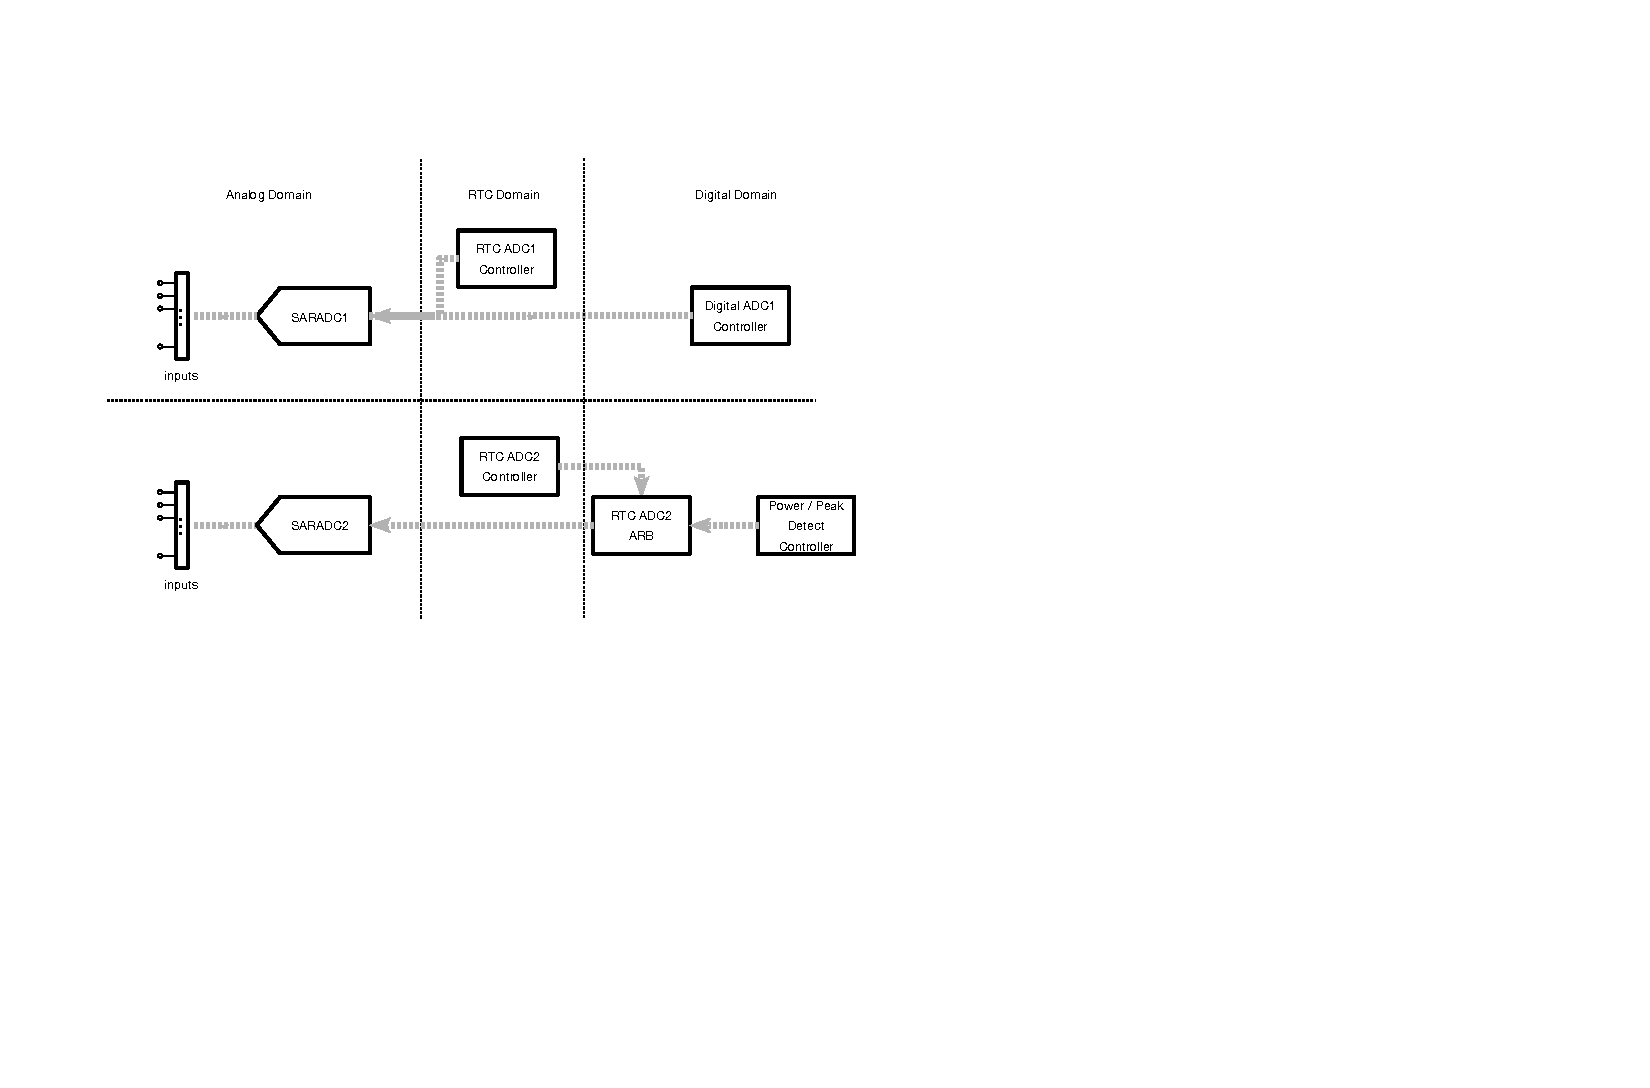
\includegraphics[width=1.0\textwidth]{25-SENSOR/figures/sar_adc_overview.pdf}
    \caption{SAR ADC Overview}
    \label{figure:sar adc overview}
\end{figure}

As shown in Figure \ref{figure:sar adc overview}, the SAR ADCs are managed by four dedicated controllers:

\begin{itemize}
   \item One digital controller: digital ADC1 controller (DIG ADC1 controller), designed for high-performance multi-channel scanning and DMA continuous conversion.
   \item Two RTC controllers: RTC ADC1 controller and RTC ADC2 controller, designed for single conversion mode and low power mode.
\item One internal controller: Power/Peak Detect Controller (PWDET controller), designed to monitor RF power. Note this controller is only for RF internal use.
\end{itemize}

\begin{tiplisting}
The DIG ADC2 controller of \chipname{} doesn't work properly and related information has been deleted in this chapter. For more information, please refer to \href{\linkprefix\linkchiperrataEN}{\chipseries{} Series SoC Errata}.
\end{tiplisting}

\subsection{Features}

The SAR ADC module has the following features:
\begin{itemize}
\item Each SAR ADC controller has its own ADC Reader module. See Figure \ref{fig:sar-adc-functional-overview}.
\item Support DIG ADC1 controller and RTC ADC1 controller to get the control of SAR ADC1 via software.
\item Support RTC ADC2 controller and PWDET controller to get the control of SAR ADC2 by the specified arbitration method via the arbiter.
\item Support 12-bit sampling resolution
\item Support sampling the analog voltages from up to 20 pins
\item RTC ADC1/2 controllers, with the following features:
    \begin{itemize}
        \item Support single conversion mode
        \item Support working in low power mode, such as in Deep-sleep mode
        \item Configurable by the ULP coprocessor
    \end{itemize}
\item DIG ADC1 controller, with the following features:
    \begin{itemize}
        \item Support multi-channel scanning
        \item Provide a mode control module, supporting single SAR ADC sampling mode
        \item Configurable scanning sequence in multi-channel scanning mode
        \item Provide two filters with configurable coefficient
        \item Support threshold monitoring. An interrupt will be triggered when the sampled value is greater than the pre-set high threshold or less than the pre-set low threshold.
        \item Support DMA
    \end{itemize}
\item PWDET controller: monitor RF power. Note this controller is only for RF internal use.
\end{itemize}


\subsection{SAR ADC Architecture}

The major components of SAR ADCs and their interconnections are shown in Figure  \ref{fig:sar-adc-functional-overview}.

\begin{figure}[H]
    \centering
    
\includegraphics[width=1.0\textwidth]{\modulefiles/figures/adc_functional_blocks_20220906.png}
    \caption{SAR ADC Architecture}
    \label{fig:sar-adc-functional-overview}
\end{figure}
\vspace{-2em}
\begin{itemize}
    \item \textcolor{red}{\textbf{—-->}}: clock signals
    \item
    \begin{tikzpicture}
\draw[rounded corners][red][dashed] (0,0) rectangle (1,0.5);
\end{tikzpicture}
: clock divider, clock mux, and the blocks the clock works for
    \end{itemize}


As shown in Figure  \ref{fig:sar-adc-functional-overview}, the SAR ADC module consists of the following components:


\begin{itemize}
    \item SAR ADC1: measures voltages from up to 10 channels.
    \item SAR ADC2: measures the voltage from 10 channels.
    \item Clock management: selects clock sources and their dividers:
            \begin{itemize}
                \item Clock sources of DIG ADC1 controller: APB\_CLK or PLL\_D2\_CLK
                \item Divided clocks of DIG ADC1 controller:
                \begin{itemize}
                    \item DIGADC\_SARCLK: operating clock for SAR ADC1, SAR ADC2, and Digital Reader1. Note that the divider (DIG\_SAR\_DIV) must be no less than 2, and the frequency of DIGADC\_SARCLK must not exceed 5 MHz. See \hyperref[fielddesc:APBSARADCSARCLKDIV]{APB\_SARADC\_SAR\_CLK\_DIV}.
                    \item DIGADC\_CLK: operating clock for DIG ADC FSM1.
                \end{itemize}
                \item Clock source of RTC ADC1/2 controllers: RTC\_FAST\_CLK
                \item Divided clock of RTC ADC1/2 controllers:
                \begin{itemize}
                    \item RTCADC\_SARCLK: operating clock for SAR ADC1, SAR ADC2, RTC Reader1, and RTC Reader2. Note that the divider (RTC\_SAR\_DIV) must be no less than 2, and the frequency of RTCADC\_SARCLK must not exceed 5 MHz.
\end{itemize}
            \end{itemize}
    \item Arbiter (ADC2\_ARBIT): this arbiter determines which controller is selected as the RTC ADC2 controller or PWDET controller. The arbiter also selects working clock for SAR ADC2 according to the authorized controller.

    \item Timer: the dedicated timer for DIG ADC1 controller, to initiate a sampling enable signal.

    \item DIG ADC FSM1: is used to
    \begin{itemize}
        \item receive the sampling enable signal from the timer.
        \item generate ADC configuration according to the pattern table.
        \item drive the Digital Reader1 module to read ADC sampling value.
        \item transfer the sampling value to the filter, and then to memory.
    \end{itemize}
    \item Filter: the filter0/1 will automatically filter the sampled ADC data for the configured channel.
    \item Threshold Monitor: the monitor0/1 will trigger a interrupt when the sampled value is greater than the pre-set high threshold or less than the pre-set low threshold.
    \item Mode control (MODE CNTL): filter the sampling signals triggered by the timer, supporting single SAR-ADC sampling.
    \item \label{block:digital-reader0} Digital Reader1 (driven by DIG ADC FSM1): reads data from SAR ADC1.
    \item RTC Controller1/2: provides sampling enable signal, drives the RTC Reader1/2 to read the sampling values from ADC, then stores the sampling data to memory.
    \item RTC Reader1/2 (driven by RTC Controller1/2): reads data from SAR ADC1/2.
\end{itemize}

\subsection{Input Signals}

In order to sample an analog signal, an SAR ADC must first select the analog pin to measure via an internal multiplexer. A summary of all the analog signals that may be sent to the SAR ADC1 or SAR ADC2 for processing are presented in Table \ref{tab:adc-inputs}.

\begin{longtable}{ |p{3cm}|C{2cm}|p{3cm}| }
    \caption{SAR ADC Input Signals}
    \label{tab:adc-inputs}
    \\\hline
    \rowcolor{lightgray}
    \textbf{Pin/Signal} & \textbf{Channel}  & \textbf{ADC Selection} \\\hline
    \endfirsthead
    \hline
    \rowcolor{lightgray}
    \textbf{Pin/Signal} & \textbf{Channel}  & \textbf{ADC Selection} \\\hline
    \endhead
    \hline
    \endfoot
    GPIO1       &  0  & \multirow{9}{*}{SAR ADC1} \\ \cline{1-2}
    GPIO2       &  1  & \\ \cline{1-2}
    GPIO3       &  2  & \\ \cline{1-2}
    GPIO4       &  3  & \\ \cline{1-2}
    GPIO5       &  4  & \\ \cline{1-2}
    GPIO6       &  5  & \\ \cline{1-2}
    GPIO7       &  6  & \\ \cline{1-2}
    GPIO8       &  7  & \\ \cline{1-2}
    GPIO9       &  8  & \\ \cline{1-2}
    GPIO10      &  9  & \multirow{13}{*}{SAR ADC2} \\ \cline{1-3}
    GPIO11      &  0  & \\ \cline{1-2}
    GPIO12      &  1  & \\ \cline{1-2}
    GPIO13      &  2  & \\ \cline{1-2}
    GPIO14      &  3  & \\ \cline{1-2}
    GPIO15      &  4  & \\ \cline{1-2}
    GPIO16      &  5  & \\ \cline{1-2}
    GPIO17      &  6  & \\ \cline{1-2}
    GPIO18      &  7  & \\ \cline{1-2}
    GPIO19      &  8  & \\ \cline{1-2}
    GPIO20      &  9  &
\end{longtable}

\subsection{ADC Conversion and Attenuation}

When the SAR ADCs convert an analog voltage, the resolution (12-bit) of the conversion spans voltage range from 0 mV to \(V_{ref}\). \(V_{ref}\) is the SAR ADC's internal reference voltage (1100 mV by design). The output value of the conversion (data) is mapped to analog voltage \(V_{data}\) using the following formula:

    \[
    V_{data} = \frac{V_{ref}}{k}\times{\frac{data}{4095}}
    \]

\(k\) is the coefficient corresponding to the configured attenuation.

In order to convert voltages larger than \(V_{ref}\), input signals can be attenuated before being input into the SAR ADCs. The supported attenuation levels are:

\begin{itemize}
    \item 0 dB (k≈100\%)
    \item 2.5 dB (k≈75\%)
    \item 6 dB (k≈50\%)
    \item 12 dB (k≈25\%)
\end{itemize}

\subsection{RTC ADC Controller}
\label{sssec:rtcadc}

The RTC ADC1/2 controllers are powered in the RTC power domain, thus
allow the SAR ADCs to conduct measurements at a low frequency with minimal power consumption. The overview of a single RTC ADC controller's function is shown in Figure \ref{figure:sar adc ctrl}.

\begin{figure}[H]
    \centering
    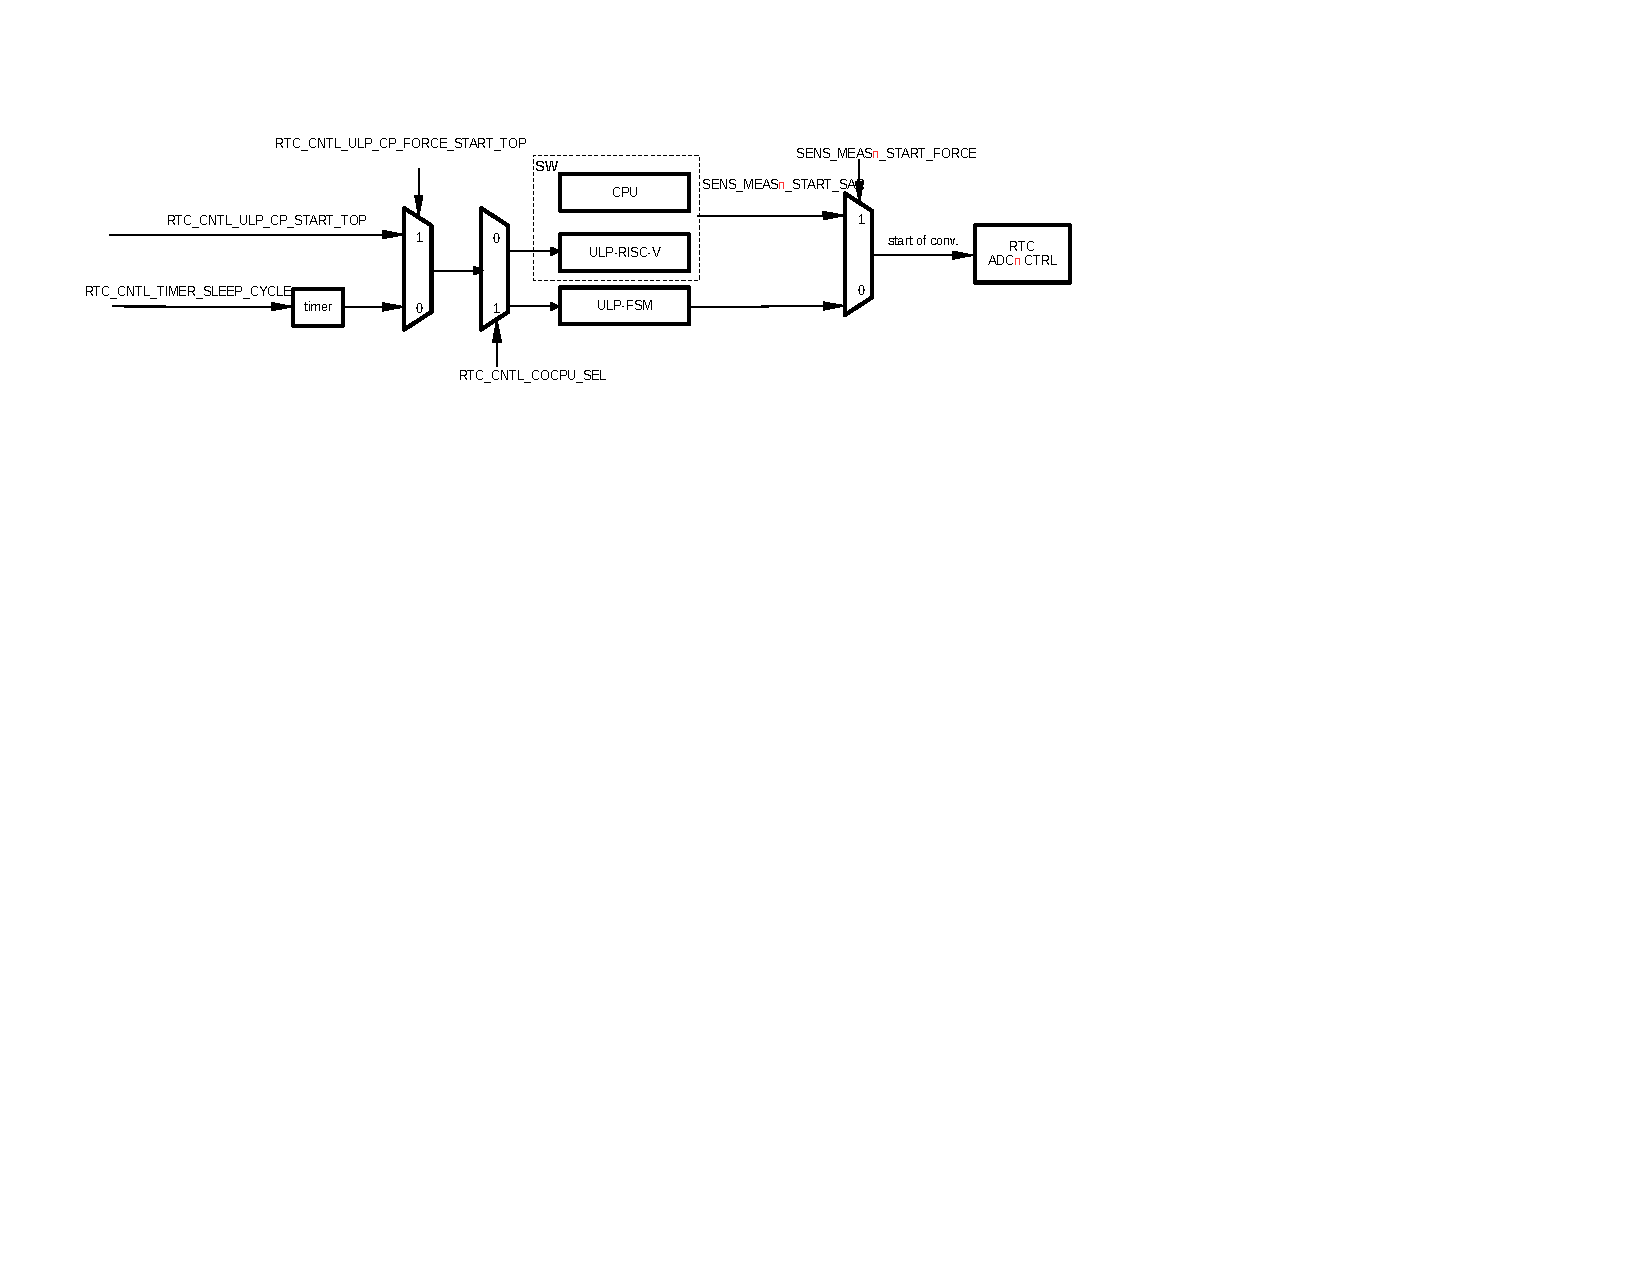
\includegraphics[width=1.0\textwidth]{25-SENSOR/figures/saradc_rtc_ctrl.pdf}
    \caption{RTC ADC Controller Overview}
    \label{figure:sar adc ctrl}
\end{figure}

Conversion is triggered by \hyperref[fielddesc:SENSMEAS1STARTSAR]{SENS\_SAR\_MEAS\regindex{n}\_START\_SAR}, and then the conversion result is stored to \hyperref[fielddesc:SENSMEAS1DATASAR]{SENS\_SAR\_MEAS\regindex{n}\_DATA\_SAR}.

The RTC ADC1/2 controllers are intertwined with the ULP coprocessor, as the ULP coprocessor has a built-in
instruction to start an ADC conversion. In many cases, the controllers need to cooperate with the ULP
coprocessor, e.g.,

\begin{itemize}
    \item When the controllers periodically monitor a channel during Deep-sleep, ULP coprocessor is the only source to trigger ADC sampling by configuring RTC registers.
    \item Continuous scanning or DMA is not supported by the controllers. However, it is possible with the help of ULP coprocessor to scan channels continuously in a sequence.
\end{itemize}

There are two ways to set the sampling channels:
\begin{itemize}
    \item Configure \hyperref[fielddesc:SENSSAR1ENPAD]{SENS\_SAR1/2\_EN\_PAD} to select sampling channels.
    \item If the ULP instruction is used to trigger a sampling, clear \hyperref[fielddesc:SENSSAR1ENPADFORCE]{SENS\_SAR1/2\_EN\_PAD\_FORCE}, to enable sampling channels by ULP instruction.
\end{itemize}

\subsection{DIG ADC Controller}

The clock of the DIG ADC1 controller is quite fast, thus the sample rate is high. For more information, see Section ADC Characteristics in \href{https://www.espressif.com/sites/default/files/documentation/esp32-s3_datasheet_en.pdf}{\chipname{} Series Datasheet}.

The DIG ADC1 controller support:

\begin{itemize}
    \item up to 12-bit sampling resolution
    \item timer-triggered multi-channel scanning
\end{itemize}

To use this timer-triggered multi-channel scanning, follow the configuration below. Note that in this mode, the scan sequence is performed according to the configuration in pattern table.

\begin{itemize}
        \item Configure  \hyperref[fielddesc:APBSARADCTIMERTARGET]{APB\_SARADC\_TIMER\_TARGET} to set the trigger target for DIG ADC timer. When the timer counting reaches two times of the pre-configured cycle number, a sampling operation is triggered. For the working clock of the timer, see Section \ref{sec:dig-adc-clock}.
        \item Configure  \hyperref[fielddesc:APBSARADCTIMEREN]{APB\_SARADC\_TIMER\_EN} to enable the timer.
        \item When the timer times out, it drives DIG ADC FSM1 to start sampling according to the pattern table.
        \item Sampled data is automatically stored in memory via DMA. An interrupt is triggered once the scan is completed.
\end{itemize}

\subsubsection{DIG ADC Clock}\label{sec:dig-adc-clock}

Two clocks can be used as the clock source for DIG ADC1 controller, depending on the configuration of \hyperref[fielddesc:APBSARADCCLKSEL]{APB\_SARADC\_CLK\_SEL}:
\begin{itemize}
    \item 0: clock off;
    \item 1: Select PLL\_D2\_CLK as the clock source. Then its divided clock DIGADC\_CLK is used as the working clock for DIG ADC1 controller;
    \item 2: Select APB\_CLK as the clock source.
\end{itemize}

If DIGADC\_CLK is selected, users can configure the divider by \hyperref[fielddesc:APBSARADCCLKMDIVNUM]{APB\_SARADC\_CLKM\_DIV\_NUM}.

Note that due to speed limits of SAR ADCs, the operating clock of Digital Reader1 and SAR ADC1 is DIGADC\_SARCLK, the frequency of which affects the sampling precision. When the frequency of DIGADC\_SARCLK is higher than 5 MHz, the sampling precision will be lowered. DIGADC\_SARCLK is divided from DIGADC\_CLK. The divider coefficient is configured by \hyperref[fielddesc:APBSARADCSARCLKDIV]{APB\_SARADC\_SAR\_CLK\_DIV}.

The ADC needs 25 DIGADC\_SARCLK clock cycles per sample, so the maximum sampling rate is limited by the DIGADC\_SARCLK frequency.

\subsubsection{DMA Support}

DIG ADC1 controller support direct memory access via peripheral DMA, which is triggered by DIG ADC timer. Users can switch the DMA data path to DIG ADC by configuring \hyperref[fielddesc:APBSARADCAPBADCTRANS]{APB\_SARADC\_APB\_ADC\_TRANS} via software. For specific DMA configuration, please refer to Chapter \ref{mod:dma} \textit{\nameref{mod:dma}}.





\subsubsection{DIG ADC FSM}

DIG ADC FSM1 drive SAR ADC1 to sample voltage in cycles according to the order and channel No. specified in the pattern table.

\begin{itemize}
    \item DIG ADC FSM1 receive the sampling enable signal from the timer.
    \item Then initiate a sampling request to SAR ADC1 according to the channel and attenuation configuration specified in the current pattern table entry pointed by the pointer (PR).
    \item Update the PR once the sampling is done.
    \begin{itemize}
        \item If the PR reaches to the entry length configured in \hyperref[fielddesc:APBSARADCSAR1PATTLEN]{APB\_SARADC\_SAR1\_PATT\_LEN}, then the PR is reset, and restarts from the first entry of the pattern table.
        \item Otherwise, the PR goes to the next entry.
    \end{itemize}
\end{itemize}


\subsubsection{Pattern Table}

DIG ADC FSM1 contain a separate pattern table configured by \hyperref[regdesc:APBSARADCSAR1PATTTAB1REG]{APB\_SARADC\_SAR1\_PATT\_TAB\regindex{x}\_REG}, where \regindex{x} represents the register No. (1 \verb+~+ 4) of the pattern table, as shown below:

\regfield{(reserved)}{8}{24}{00000000}%
\regfield{cmd0}{6}{18}{{0x{}0000}}%
\regfield{cmd1}{6}{12}{{0x{}0000}}%
\regfield{cmd2}{6}{6}{{0x{}0000}}%
\regfield{cmd3}{6}{0}{{0x{}0000}}%
\begin{regdesc}\begin{reglist}
\item [cmd \regindex{n} (\regindex{n} = 0 - 3)] represents pattern table entries 0 \verb+~+ 3.
\end{reglist}\end{regdesc}
\vspace{-2em}
\begin{figure}[H]
    \centering
    \caption{APB\_SARADC\_SAR1\_PATT\_TAB1\_REG and Pattern Table Entry 0 - Entry 3}
    \label{fig:pattern-tab-1}
\end{figure}

\regfield{(reserved)}{8}{24}{00000000}%
\regfield{cmd4}{6}{18}{{0x{}0000}}%
\regfield{cmd5}{6}{12}{{0x{}0000}}%
\regfield{cmd6}{6}{6}{{0x{}0000}}%
\regfield{cmd7}{6}{0}{{0x{}0000}}%
\begin{regdesc}\begin{reglist}
\item [cmd \regindex{n} (\regindex{n} = 4 - 7)] represents pattern table entries 4 \verb+~+ 7.
\end{reglist}\end{regdesc}
\vspace{-2em}
\begin{figure}[H]
    \centering
    \caption{APB\_SARADC\_SAR1\_PATT\_TAB2\_REG and Pattern Table Entry 4 - Entry 7}
    \label{fig:pattern-tab-2}
\end{figure}

\regfield{(reserved)}{8}{24}{00000000}%
\regfield{cmd11}{6}{18}{{0x{}0000}}%
\regfield{cmd10}{6}{12}{{0x{}0000}}%
\regfield{cmd9}{6}{6}{{0x{}0000}}%
\regfield{cmd8}{6}{0}{{0x{}0000}}%
\begin{regdesc}\begin{reglist}
\item [cmd \regindex{n} (\regindex{n} = 8 - 11)] represents pattern table entries 8 \verb+~+ 11.
\end{reglist}\end{regdesc}
\vspace{-2em}
\begin{figure}[H]
    \centering
    \caption{APB\_SARADC\_SAR1\_PATT\_TAB3\_REG and Pattern Table Entry 8 - Entry 11}
    \label{fig:pattern-tab-3}
\end{figure}

\regfield{(reserved)}{8}{24}{00000000}%
\regfield{cmd15}{6}{18}{{0x{}0000}}%
\regfield{cmd14}{6}{12}{{0x{}0000}}%
\regfield{cmd13}{6}{6}{{0x{}0000}}%
\regfield{cmd12}{6}{0}{{0x{}0000}}%
\begin{regdesc}\begin{reglist}
\item [cmd \regindex{n} (\regindex{n} = 12 - 15)] represents pattern table entries 12 \verb+~+ 15.
\end{reglist}\end{regdesc}
\vspace{-2em}
\begin{figure}[H]
    \centering
    \caption{APB\_SARADC\_SAR1\_PATT\_TAB4\_REG and Pattern Table Entry 12 - Entry 15}
    \label{fig:pattern-tab-4}
\end{figure}

Each register consists of four 6-bit pattern table entries. Each entry is composed of two fields that contain ADC channel and attenuation information, as shown in Table \ref{tab:pattern-table-register}.


\begin{figure}[H]
\centering
\regfield{ch\_sel}{4}{2}{{xx}}%
\regfield{atten}{2}{0}{xx}%
\end{figure}
\vspace{-2em}
\begin{figure}[H]
    \centering
    \caption{Pattern Table Entry}
    \label{tab:pattern-table-register}
\end{figure}
\vspace{-2em}
\begin{regdesc}\begin{reglist}
\item [atten] Attenuation. 0: 0 dB; 1: 2.5 dB; 2: 6 dB; 3: 12 dB.
\item [ch\_sel] ADC channel, see Table \ref{tab:adc-inputs}.
\end{reglist}\end{regdesc}

\subsubsection{Configuration Example for Multi-Channel Scanning}

In this example, the following channels are selected for multi-channel scanning for SAR ADC1:
\begin{itemize}
    \item Channel 2, with the attenuation of 12 dB. See Figure \ref{fig:cmd-config-1}.
    \item Channel 0, with the attenuation of 2.5 dB. See Figure \ref{fig:cmd-config-2}.
\end{itemize}

The detailed configuration is as follows:
\begin{itemize}
    \item Configure SAR ADC1:
    \begin{itemize}
        \item Configure the first pattern table entry (cmd0, \hyperref[regdesc:APBSARADCSAR1PATTTAB1REG]{APB\_SARADC\_SAR1\_PATT\_TAB1\_REG}[5:0]):

\centering
\regfield{ch\_sel}{4}{2}{{2}}%
\regfield{atten}{2}{0}{3}%
\reglabel{}\regnewline%
\begin{regdesc}\begin{reglist}
\begin{figure}[H]
    \centering
    \caption{SAR ADC1 cmd0 Configuration}
    \label{fig:cmd-config-1}
\end{figure}
\vspace{-2em}
\item [atten] write the value of 3 to this field, to set the attenuation to 12 dB.
\item [ch\_sel] write the value of 2 to this field, to select channel 2 (see Table \ref{tab:adc-inputs}).
\end{reglist}\end{regdesc}
\end{itemize}

\begin{itemize}
    \item Configure the second pattern table entry (cmd1, \hyperref[regdesc:APBSARADCSAR1PATTTAB1REG]{APB\_SARADC\_SAR1\_PATT\_TAB1\_REG}[11:6]):

\centering
\regfield{ch\_sel}{4}{2}{{0}}%
\regfield{atten}{2}{0}{1}%
\reglabel{}\regnewline%
\begin{regdesc}\begin{reglist}
\begin{figure}[H]
    \centering
    \caption{SAR ADC1 cmd1 Configuration}
    \label{fig:cmd-config-2}
\end{figure}
\vspace{-2em}
\item [atten] write the value of 1 to this field, to set the attenuation to 2.5 dB.
\item [ch\_sel] write the value of 0 to this field, to select channel 0 (see Table \ref{tab:adc-inputs}).
\end{reglist}\end{regdesc}
\end{itemize}
\end{itemize}




\begin{itemize}
    \item Configure \hyperref[fielddesc:APBSARADCSAR1PATTLEN]{APB\_SARADC\_SAR1\_PATT\_LEN} to 1, i.e., set pattern table length to (this value + 1 = 2). Then pattern table entries cmd0 and cmd1 for SAR ADC1 will be used.
    \item Enable the timer, then DIG ADC1 controller start scanning the channel 2 and channel 0 of SAR ADC1 in cycles, as configured in the pattern table entries.
\end{itemize}

\subsubsection{DMA Data Format}

The SAR ADCs eventually pass 32-bit data to the DMA, see the figure below.

\begin{figure}[H]
\centering
\regfield{reserved}{16}{17}{{xx}}%
\regfield{ch\_sel}{3}{13}{{xxx}}%
\regfield{reserved}{1}{12}{{x}}%
\regfield{data}{12}{0}{xx}%
\end{figure}
\vspace{-2em}
\begin{figure}[H]
    \centering
    \caption{DMA Data Format}
    \label{fig:dma-data-format}
\end{figure}
\vspace{-2em}
\begin{regdesc}\begin{reglist}
\item [data] SAR ADC data, 12-bit
\item [ch\_sel] Channel, 3-bit
\end{reglist}\end{regdesc}


\subsubsection{ADC Filters}

The DIG ADC1 controller provide two filters for automatic filtering of sampled ADC data. Both filters can be configured to any two channels of SAR ADC and then filter the sampled data for the target channel. The filter's formula is shown below:

\[data_{cur} = \frac{(k-1)data_{prev}}{k}+\frac{data_{in}}{k}+0.5\]

\begin{itemize}
    \item \(data_{cur}\): the filtered data value.
    \item \(data_{in}\): the sampled data value from the SAR ADC.
    \item \(data_{prev}\): the last filtered data value.
    \item \(k\): the filter coefficient.
\end{itemize}

The filters are configured as follows:
\begin{itemize}
\item Configure \hyperref[fielddesc:APBSARADCFILTERCHANNEL1]{APB\_SARADC\_FILTER\_CHANNEL\regindex{x}} to select the SAR ADC channel for filter \regindex{x};
\item Configure \hyperref[fielddesc:APBSARADCFILTERCHANNEL1]{APB\_SARADC\_FILTER\_FACTOR\regindex{x}} to set the coefficient for filter \regindex{x}.
\end{itemize}


Note that \regindex{x} is used here as the placeholder of filter index. 0: filter 0; 1: filter 1.

\subsubsection{Threshold Monitoring}

DIG ADC1 controller contain two threshold monitors that can be configured to monitor on any channel of SAR ADC1. A high threshold interrupt is triggered when the ADC sample value is larger than the pre-configured high threshold, and a low threshold interrupt is triggered if the sample value is lower than the pre-configured low threshold.

The configuration of threshold monitoring is as follows:
\begin{itemize}
    \item Set \hyperref[fielddesc:APBSARADCTHRESALLEN]{APB\_SARADC\_THRES\regindex{x}\_EN} to enable threshold monitor \regindex{x}.
    \item Configure \hyperref[fielddesc:APBSARADCTHRES1LOW]{APB\_SARADC\_THRES\regindex{x}\_LOW} to set a low threshold.
    \item Configure \hyperref[fielddesc:APBSARADCTHRES1LOW]{APB\_SARADC\_THRES\regindex{x}\_HIGH} to set a high threshold.
    \item Configure \hyperref[fielddesc:APBSARADCTHRES1LOW]{APB\_SARADC\_THRES\regindex{x}\_CHANNEL} to select the SAR ADC and the channel to monitor.
\end{itemize}

Note that \regindex{x} is used here as the placeholder of monitor index. 0: monitor 0; 1: monitor 1.



\subsection{SAR ADC2 Arbiter}

SAR ADC2 can be controlled by two controllers, namely, RTC ADC2 controller and PWDET controller. To avoid any possible conflicts and to improve the efficiency of SAR ADC2, \chipname{} provides an arbiter for SAR ADC2. The arbiter supports fair arbitration and fixed priority arbitration.

\begin{itemize}
    \item Fair arbitration mode (cyclic priority arbitration) can be enabled by clearing  \hyperref[fielddesc:APBSARADCADCARBFIXPRIORITY]{APB\_SARADC\_ADC\_ARB\_FIX\_\\PRIORITY}.
    \item In fixed priority arbitration, users can set \hyperref[fielddesc:APBSARADCADCARBRTCPRIORITY]{APB\_SARADC\_ADC\_ARB\_RTC\_PRIORITY} (for RTC ADC2 controller) or \hyperref[fielddesc:APBSARADCADCARBWIFIPRIORITY]{APB\_SARADC\_ADC\_ARB\_\\WIFI\_PRIORITY} (for PWDET controller), to configure the priorities for these controllers. A larger value indicates a higher priority.
\end{itemize}

The arbiter ensures that a higher priority controller can always start a conversion (sample) when required, regardless of whether a lower priority controller already has a conversion in progress. If a higher priority controller starts a conversion whilst the ADC already has a conversion in progress from a lower priority controller, the conversion in progress will be interrupted (stopped). The higher priority controller will then start its conversion. A lower priority controller will not be able to start a conversion whilst the ADC has a conversion in progress from a higher priority controller.

Therefore, certain data flags are embedded into the output data value to indicate whether the conversion is valid or not.

\begin{itemize}
    \item The data flag for RTC ADC2 controller is the higher two bits of \hyperlink{fielddesc:SENSMEAS2DATASAR}{SENS\_MEAS2\_DATA\_SAR}.
    \begin{itemize}
        \item 2'b10: Conversion is interrupted.
        \item 2'b01: Conversion is not started.
        \item 2'b00: The data is valid.
    \end{itemize}

    \item The data flag for PWDET controller is the higher two bits of the sampling result.

    \begin{itemize}
        \item 2'b10: Conversion is interrupted.
        \item 2'b01: Conversion is not started.
        \item 2'b00: The data is valid.
    \end{itemize}
\end{itemize}
Users can configure  \hyperref[fielddesc:APBSARADCADCARBGRANTFORCE]{APB\_SARADC\_ADC\_ARB\_GRANT\_FORCE} to mask the arbiter, and set \hyperref[fielddesc:APBSARADCADCARBWIFIFORCE]{APB\_SARADC\_ADC\_\\ARB\_WIFI\_FORCE} or \hyperref[fielddesc:APBSARADCADCARBRTCFORCE]{APB\_SARADC\_ADC\_ARB\_RTC\_FORCE} to authorize corresponding controllers.

\begin{tiplisting}
\vspace{-2em}
\begin{itemize}
    \item When the arbiter is masked, only one of the above APB\_SARADC\_ADC\_ARB\_XXX\_FORCE bits can be set to 1.
    \item The arbiter uses APB\_CLK as its clock source. When the clock frequency is 8 MHz or lower, the arbiter must be masked.
    \item In sleep mode, the \hyperref[fielddesc:SENSSAR2RTCFORCE]{SENS\_SAR2\_RTC\_FORCE} in register \hyperref[regdesc:SENSSARMEAS2MUXREG]{SENS\_SAR\_MEAS2\_MUX\_REG} should be set to 1, masking the arbiter and all the signals from controllers except the RTC controllers.
\end{itemize}
\end{tiplisting}


\section{Temperature Sensor}\label{sec:tsensor}
\subsection{Overview}

\chipname{} provides a temperature sensor to monitor temperature changes inside the chip in real time.

\subsection{Features}
The temperature sensor has the following features:
\begin{itemize}
    \item Monitored in real time by ULP coprocessor when in low-power mode
    \item Triggered by software or by ULP coprocessor
    \item Configurable temperature offset based on the environment, to improve the accuracy
    \item Adjustable measurement range
\end{itemize}

\subsection{Functional Description}
\begin{figure}[H]
    \centering
    
\includegraphics[width=1.0\textwidth]{\modulefiles/figures/tsensor_struct.pdf}
    \caption{Temperature Sensor Overview}
    \label{fig:tsensor-struct}
\end{figure}
As shown in Figure \ref{fig:tsensor-struct}, the temperature sensor can be started by software or by ULP coprocessor:
\begin{itemize}
   \item Started by software, i.e. by CPU or ULP-RISC-V configuring related registers:
    \begin{itemize}
        \item Set \hyperref[fielddesc:SENSTSENSPOWERUPFORCE]{SENS\_TSENS\_POWER\_UP\_FORCE} and \hyperref[fielddesc:SENSTSENSPOWERUP]{SENS\_TSENS\_POWER\_UP} to enable the temperature sensor.
        \item Set \hyperref[fielddesc:SENSFORCEXPDSAR]{SENS\_FORCE\_XPD\_SAR} to force SAR ADC power on, and set \hyperref[fielddesc:SENSTSENSCLKEN]{SENS\_TSENS\_CLK\_EN} to enable temperature sensor clock.
        \item Wait for a while, then configure \hyperref[fielddesc:SENSTSENSDUMPOUT]{SENS\_TSENS\_DUMP\_OUT}. The output value gradually approaches the actual temperature linearly as the measurement time increases.

        \item Wait for \hyperref[fielddesc:SENSTSENSREADY]{SENS\_TSENS\_READY}, and read the conversion result from \hyperref[fielddesc:SENSTSENSOUT]{SENS\_TSENS\_OUT}.
    \end{itemize}
    \item Started by ULP-FSM:
    \begin{itemize}
        \item Clear \hyperref[fielddesc:SENSTSENSPOWERUPFORCE]{SENS\_TSENS\_POWER\_UP\_FORCE}.
        \item ULP-FSM has a built-in instruction for temperature sampling. Executing the instruction can easily complete temperature sampling, see Chapter \ref{mod:ulp} \textit{\nameref{mod:ulp}}.
    \end{itemize}
\end{itemize}



The actual temperature (°C) can be obtained by converting the output of temperature sensor via the following formula:

\begin{centering}
        T(°C) = 0.4386 * VALUE – 27.88 * offset – 20.52\\
\end{centering}

VALUE in the formula is the output of the temperature sensor, and the offset is determined by the temperature offset. The temperature offset varies in different actual environment (the temperature range). For details, refer to Table \ref{tab:tsensor-dac}.

\begin{longtable}[c]{|l|r|}
    \caption{Temperature Measurement Range and Offset}
    \label{tab:tsensor-dac}
    \\\hline
    \rowcolor{lightgray}
    \textbf{Temperature Measurement Range (°C)}   & \textbf{Temperature Offset} \\\hline
    50 \verb+~+ 125 &  –2 \\\hline
    20 \verb+~+ 100 &  –1 \\\hline
    –10 \verb+~+ 80 &  0 \\\hline
    –30 \verb+~+ 50 &  1 \\\hline
    –40 \verb+~+ 20 &  2 \\\hline
\end{longtable}

\section{Interrupts}

\begin{itemize}
   \item \label{interreupt:APBSARADCTHRESxHIGHINT} APB\_SARADC\_THRES\regindex{x}\_HIGH\_INT: Triggered when the sampling value is higher than the high threshold of monitor \regindex{x}.
    \item \label{interreupt:APBSARADCTHRESxLOWINT} APB\_SARADC\_THRES\regindex{x}\_LOW\_INT: Triggered when the sampling value is lower than the low threshold of monitor \regindex{x}.
   \item \label{interreupt:SARADCDONEINT1}APB\_SARADC\_ADC1\_DONE\_INT: Triggered when SAR ADC1 completes one data conversion.
\end{itemize}
For the interrupts routed to ULP-RISC-V, please refer to Section ULP-RISC-V Interrupts in Chapter \ref{mod:ulp} \textit{\nameref{mod:ulp}}.

\hypertarget{sensor-reg-summ}{}
\section{Register Summary}

\begin{itemize}
   \item SENSOR (ALWAYS\_ON) represents the registers, which will not be reset due to the power down of RTC\_PERI domain. See Chapter \ref{mod:lowpowm} \textit{\nameref{mod:lowpowm}}.
    \item SENSOR (RTC\_PERI) represents the registers, which will be reset due to the power down of RTC\_PERI domain. See Chapter \ref{mod:lowpowm} \textit{\nameref{mod:lowpowm}}.
    \item SENSOR (DIG\_PERI) represents the registers, which will be reset due to the power down of digital domain. See Chapter \ref{mod:lowpowm} \textit{\nameref{mod:lowpowm}}.
\end{itemize}

\subsection{SENSOR (ALWAYS\_ON) Register Summary}

The addresses in this section are relative to the [Low Power Management] base address provided in Table \ref{tab:sysmem-base-address} in Chapter \ref{mod:sysmem} \textit{\nameref{mod:sysmem}}.

\subfile{\modulefiles/25-SENSOR-always-on-reg-summ__EN}

\subsection{SENSOR (RTC\_PERI) Register Summary}

The addresses in this section are relative to the [Low Power Management base address + 0x{}800] provided in Table \ref{tab:sysmem-base-address} in Chapter \ref{mod:sysmem} \textit{\nameref{mod:sysmem}}.

The abbreviations given in Column \textbf{Access} are explained in Section \hyperref[glossary-access-types]{\textit{Access Types for Registers}}.

\subfile{\modulefiles/25-SENSOR-saradc-reg-summ__EN}

\subsection{SENSOR (DIG\_PERI) Register Summary}

The addresses in this section are relative to the [ADC controller base address] provided in Table \ref{tab:sysmem-base-address} in Chapter \ref{mod:sysmem} \textit{\nameref{mod:sysmem}}.

The abbreviations given in Column \textbf{Access} are explained in Section \hyperref[glossary-access-types]{\textit{Access Types for Registers}}.

\subfile{\modulefiles/25-SENSOR-apb-saradc-reg-summ__EN}


\section{Registers}
\label{section:registers}

\subsection{SENSOR (ALWAYS\_ON) Registers}

The addresses in this section are relative to the [Low Power Management] base address provided in Table \ref{tab:sysmem-base-address} in Chapter \ref{mod:sysmem} \textit{\nameref{mod:sysmem}}.

\subfile{\modulefiles/25-SENSOR-always-on-reg__EN}

\subsection{SENSOR (RTC\_PERI) Registers}

The addresses in this section are relative to the [Low Power Management base address + 0x{}800] provided in Table \ref{tab:sysmem-base-address} in Chapter \ref{mod:sysmem} \textit{\nameref{mod:sysmem}}.

\subfile{\modulefiles/25-SENSOR-saradc-reg__EN}

\subsection{SENSOR (DIG\_PERI) Registers}

The addresses in this section are relative to the [ADC controller base address] provided in Table \ref{tab:sysmem-base-address} in Chapter \ref{mod:sysmem} \textit{\nameref{mod:sysmem}}.

\subfile{\modulefiles/25-SENSOR-apb-saradc-reg__EN}


\end{document}
